\section{Informal Description of Subject Behavior Execution}


%ME: for now i have put all descriptions of SBD model elements into chapter 2b
%all aspects concerning execution are to be re put into this chapter


Before sending a message, the values of the parameters to be transmitted need to be determined. In case the message parameters are simple data types, the required values are taken from local variables or business objects of the sending subject, respectively. In the case of business objects, a current instance of a business object is transferred as a message parameter.

The sending subject attempts to send the message to the target subject and store it in its input pool. Depending on the described configuration and status of the input pool, the message is either immediately stored or the sending subject is blocked until delivery of the message is possible.

%The blocking of subjects when attempting to send can be monitored over time with the so-called timeout. The example in Figure \ref{fig:sendstatetimer} shows with 'Timeout: 24 h' an additional state transition which occurs when within 24 hours one of the two messages cannot be sent. If a value of zero is specified for the timeout, the process immediately follows the timeout path when the alternative message delivery fails.

\subsection{Receiving Messages}

Analogously to sending, the receiving procedure is divided into two phases, which run inversely to send.

The first step is to verify whether the expected message is ready for being picked up. In the case of synchronous messaging, it is checked whether the sending subject offers the message. In the asynchronous version, it is checked whether the message has already been stored in the input pool. If the expected message is accessible in either form, it is accepted, and in a second step, the corresponding state transition is performed. This leads to a takeover of the message parameters of the accepted message to local variables or business objects of the receiving subject. In case the expected message is not ready, the receiving subject is blocked until the message arrives and can be accepted.

In a certain state, a subject can expect alternatively multiple messages. In this case, it is checked whether any of these messages are available and can be accepted. The test sequence is arbitrary unless message priorities are defined. In this case, an available message with the highest priority is accepted. However, all other messages remain available (e.g., in the input pool) and can be accepted in other receive states.

Figure \ref{fig:receivestate} shows a receive state of the subject 'employee' which is waiting for the answer regarding a business trip request. The answer may be an approval or a rejection.

\begin{figure*}[htbp]
	\centering
	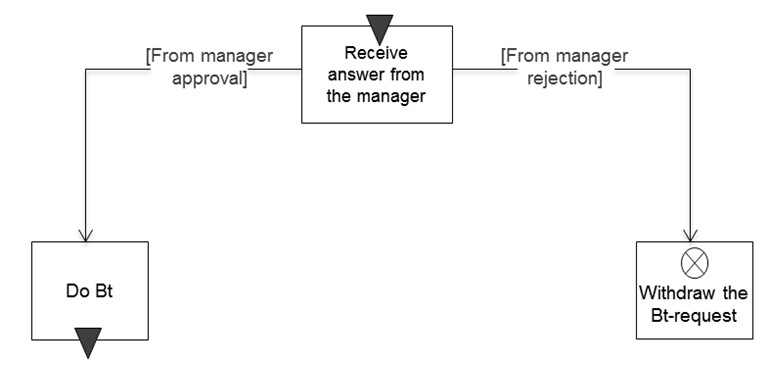
\includegraphics[width=0.7\linewidth]{Figures/Ontology/SubjectBehavior/ReceiveState}
	\caption[Example of alternative receiving]{Example of alternative receiving}
	\label{fig:receivestate}
\end{figure*}

Just as with sending messages, also receiving messages can be monitored over time. If none of the expected messages are available and the receiving subject is therefore blocked, a time limit can be specified for blocking. After the specified time has elapsed, the subject will execute the transition as it is defined for the timeout period. The duration of the time limit may also be dynamic, in the sense that at the end of a process instance the process stakeholders assigned to the subject decide that the appropriate transition should be performed. We then speak of a manual timeout.

\subsection{Sending Messages}




%\begin{figure}[htbp]
%	\centering
%	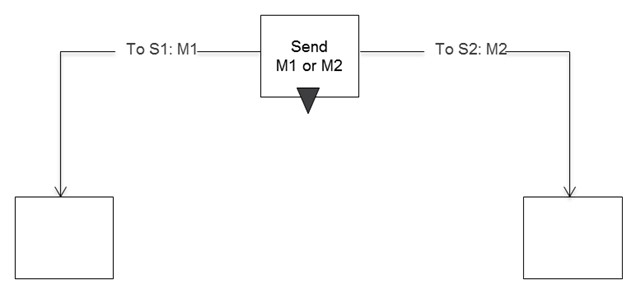
\includegraphics[width=0.7\linewidth]{Figures/Ontology/SubjectBehavior/sendState}
%	\caption[Example of alternative sending]{Example of alternative sending}
%	\label{fig:sendstate}
%\end{figure}

%By specifying priorities, the order of sending can be influenced. For example, it can be determined that the message M1 to S1 has a higher priority than the message M2 to S2. Using this specification, the sending subject starts with sending message M1 to S1 and then tries only in case of failure to send message M2 to S2. In case of message M2 can also not be sent to the subject S2, the attempts to send start from the beginning.

%The blocking of subjects when attempting to send can be monitored over time with the so-called timeout. The example in Figure \ref{fig:sendstatetimer} shows with 'Timeout: 24 h' an additional state transition which occurs when within 24 hours one of the two messages cannot be sent. If a value of zero is specified for the timeout, the process immediately follows the timeout path when the alternative message delivery fails.

%\begin{figure*}[htbp]
%	\centering
%	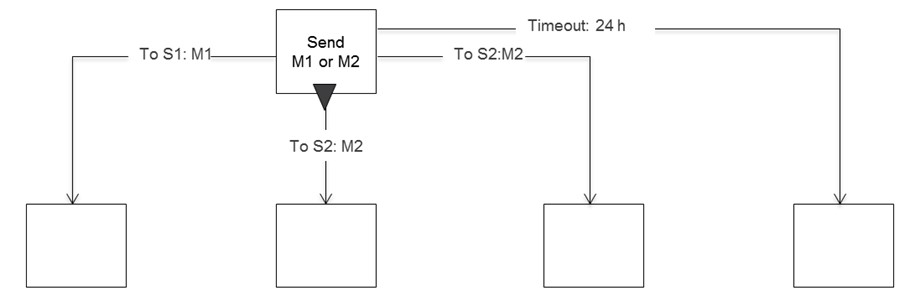
\includegraphics[width=0.7\linewidth]{Figures/Ontology/SubjectBehavior/SendSTateTimer}
%	\caption[Send using time monitoring]{Send using time monitoring}
%	\label{fig:sendstatetimer}
%\end{figure*}